% ==============================================================================
% Chapter 1: Introduction
% ==============================================================================
\chapter{Introduction}
\label{ch:intro}

\section{Background}
\label{sec:background}

\subsection{Motivation and Need}
Urban traffic congestion has emerged as one of the most critical socio-economic and environmental challenges facing modern developing economies. In rapidly expanding metropolitan regions such as the National Capital Region (NCR) of India, arterial corridors experience unprecedented traffic densities characterized by severe saturation, non-lane-based vehicle interactions, and profound modal heterogeneity \cite{ref_tomtom2023, ref_irc106}. The Delhi--Gurgaon arterial corridor along National Highway 48 (NH-48), specifically the critical stretch spanning Rajiv Chowk, IFFCO Chowk, and Signature Tower, represents one of the busiest and most economically vital transport arteries in South Asia, carrying in excess of 250,000 passenger car units (PCU) on peak weekdays \cite{ref_delhidataset}. 

Despite significant capital investments in multi-lane physical road infrastructure and grade-separated flyovers, surface-level intersections and arterial merge zones continue to suffer from catastrophic vehicular gridlock. The predominant cause of this congestion lies in the fundamental operational limitations of prevailing traffic signal control infrastructure \cite{ref_roess2010}. The vast majority of municipal traffic lights across Indian cities continue to operate on static, pre-timed (fixed-time) signal plans designed using historical Webster's formulations or rigid cyclic time-of-day splits. These open-loop controllers lack sensory feedback mechanisms, allocating uniform green durations irrespective of real-time directional arrival surges, downstream blockages, or sudden bottleneck incidents. 

Even where localized vehicle-actuated systems or inductive loop detectors have been piloted, traditional centralized systems (such as SCOOT or SCATS) prove exceptionally fragile, cost-prohibitive, and conceptually misaligned with the realities of Indian roadways \cite{ref_scats1980}. First, inductive loop sensors cut into the asphalt degrade rapidly under Indian climate extremes and overloaded commercial axle loads. Second, conventional urban traffic control architectures rely on the critical assumption of strict lane discipline, homogeneous passenger car fleets, and orderly queuing behavior. In contrast, Indian urban traffic is intensely heterogeneous: over 55\% to 70\% of vehicular volume comprises two-wheelers (motorcycles and scooters) and three-wheelers (auto-rickshaws), which engage in continuous sublane filtering, lateral swarming, and non-lane queueing at signal approaches \cite{ref_pune_dataset, ref_iisc_bmd45}. When a controller treats a high-occupancy state transport bus carrying 60 passengers identically to five filtering motorized two-wheelers occupying the same spatial footprint, the resulting signal timing drastically misallocates scarce green clearance capacity.

Recent advances in artificial intelligence offer two transformative paradigms capable of overcoming these systemic failures:
\begin{enumerate}
    \item \textbf{Edge Computer Vision for Heterogeneous Traffic Perception}: Deep convolutional object detection frameworks, specifically the real-time YOLO (You Only Look Once) architecture \cite{ref_yolov8}, enable non-intrusive CCTV-based vehicle detection. When coupled with specialized Indian vehicle taxonomies such as the Indian Institute of Science Bengaluru Mobility Dataset (IISc AIM BMD-45) and Indian Roads Congress (IRC:106-1990) Passenger Car Unit (PCU) conversions, vision systems can calculate true dynamic road capacity demand in real time.
    \item \textbf{Multi-Agent Deep Reinforcement Learning (MARL)}: The arterial traffic control problem is fundamentally a decentralized multi-agent coordination challenge. Isolated single-intersection reinforcement learning agents suffer from acute environmental non-stationarity, frequently creating downstream shockwaves by clearing one junction only to dump overwhelming platoons into an already gridlocked neighbor. Multi-Agent Proximal Policy Optimization (MAPPO) with Centralized Training and Decentralized Execution (CTDE) enables adjacent traffic signal controllers along a multi-intersection corridor to learn collaborative policies, establishing progressive ``green waves'' without requiring brittle inter-site physical wiring or costly cloud dependencies \cite{ref_mappo2022}.
\end{enumerate}

This project, titled \textit{Multi-Agent Deep Reinforcement Learning for Adaptive Traffic Signal Control in Indian Corridors}, bridges the gap between theoretical reinforcement learning and deployable, real-world Indian traffic systems. By replacing fragile microscopic simulators with a data-driven Neural Traffic World Model trained on empirical Indian sensor data, and integrating live CCTV edge perception with a cooperative MAPPO policy, this work delivers an autonomous, zero-cloud adaptive traffic signal digital twin.

\section{Problem Definition and Objectives}
\label{sec:problem_def_obj}

\subsection{Problem Definition}
The objective of this research is to design, model, implement, and benchmark an autonomous, edge-compatible Multi-Agent Deep Reinforcement Learning system for adaptive traffic signal control on multi-intersection Indian arterial corridors. The system must ingest heterogeneous camera feeds or sensor streams, classify mixed traffic according to IRC:106 PCU equivalents, predict spatial corridor queuing dynamics using a data-driven Neural World Model, and execute coordinated signal phase decisions across interconnected intersections to minimize cumulative commuter delay, reduce stop frequency, and prevent gridlock.

This technical challenge is decomposed into four foundational engineering problems:
\begin{itemize}
    \item \textbf{Handling Extreme Heterogeneity and Non-Lane Queuing}: Traditional detectors count vehicle units. The perception engine must identify two-wheelers, auto-rickshaws, passenger cars, buses, and commercial trucks from CCTV video and compute continuous PCU loads without relying on marked lane markings.
    \item \textbf{Multi-Intersection Non-Stationarity and Coordination}: Individual signal controllers along an arterial corridor affect one another through vehicular platoon discharge. The control algorithm must eliminate competitive or selfish switching and foster decentralized coordination.
    \item \textbf{Eliminating the Fragility of Microscopic Simulation}: Conventional RL approaches rely on the microscopic SUMO (Simulation of Urban MObility) simulator running over TCP/IP sockets, which experiences frequent TraCI connection timeouts, heavy CPU burdens, and poor calibration to Indian filtering dynamics. A lightweight, data-driven surrogate simulator is required.
    \item \textbf{Failsafe and Safety-Constrained Real-Time Execution}: Signal transitions must strictly enforce civil safety clearance standards, including minimum green intervals, yellow amber warnings, and all-red clearance intervals to prevent vehicular collisions.
\end{itemize}

\subsection{Measurable Objectives}
To address this problem, the project establishes five clear, measurable technical objectives:
\begin{enumerate}
    \item \textbf{Objective 1 -- Multi-Agent Policy Architecture}: Formulate and train a Multi-Agent Proximal Policy Optimization (MAPPO) framework operating under Centralized Training with Decentralized Execution (CTDE), controlling 3 to 4 signalized intersections along the NH-48 corridor with parameter sharing.
    \item \textbf{Objective 2 -- Real-World Data Ingestion \& Heterogeneous Perception}: Ingest empirical Indian traffic datasets (IIT Delhi 40-day sensor density, Mendeley Pune turning counts, and IISc AIM BMD-45 taxonomy) to map vehicle classes to IRC:106 PCU weights ($0.5$ for 2W, $1.0$ for Auto/Car, $3.0$ for Bus/Truck) at an edge inference throughput exceeding 30 frames per second.
    \item \textbf{Objective 3 -- Simulator-Free Deep Neural World Model}: Train a surrogate Deep Residual Multi-Task Dynamics Model capable of predicting next corridor states $\Delta s_t$ and IRC PCU cost rewards $r_t$ with a normalized state Mean Squared Error (MSE) below $0.005$, executing at over 100 simulation steps per second without SUMO/TraCI dependencies.
    \item \textbf{Objective 4 -- Quantitative Delay \& Queue Reduction}: Demonstrate that the trained MAPPO policy reduces average vehicular waiting delay by at least 20\% and increases arterial corridor throughput by at least 12\% compared to standard fixed-time cyclic controllers under peak rush-hour demand profiles.
    \item \textbf{Objective 5 -- End-to-End Live Video Actuation Visual Dashboard}: Develop an operational edge testing framework and interactive telemetry dashboard capable of ingesting live webcam/RTSP feeds or recorded CCTV video, rendering dynamic 3-color (Red, Yellow, Green) signal actuators, and verifying physical phase transitions.
\end{enumerate}

Table \ref{tab:objectives_mapping} maps each defined objective to its target quantitative metric and validation methodology.

\begin{table}[htbp]
\centering
\small
\caption{Project objectives, target metrics, and verification methods}
\label{tab:objectives_mapping}
\begin{tabularx}{\textwidth}{|p{3.8cm}|p{4.8cm}|X|}
\hline
\textbf{Objective} & \textbf{Target Metric} & \textbf{Verification Method} \\ \hline
1. Multi-Agent Policy Architecture & Parameter-shared MAPPO; 22-dim local obs; 66-dim global state & Convergence of policy return across 30,000 corridor timesteps \\ \hline
2. Heterogeneous Perception & Real-time YOLOv8; 5 Indian classes; $\ge 30$ FPS on CPU & Bounding box inference and PCU calculation on CCTV footage \\ \hline
3. Neural World Model & State MSE $< 0.005$; Reward MSE $< 0.05$; $> 100$ FPS & Offline validation on 10,800 unseen empirical Delhi transitions \\ \hline
4. Delay \& Queue Reduction & $\ge 20\%$ delay reduction; $\ge 12\%$ throughput gain in peak & 6-scenario benchmark vs.\ Fixed-Time and Random baselines \\ \hline
5. Live Vision Actuation & End-to-end video-to-light latency $< 50$ ms; strict Red/Yellow/Green & Hardware camera integration test and interactive web dashboard \\ \hline
\end{tabularx}
\end{table}

\section{Social \& Environmental Relevance}
\label{sec:social_env}
The societal and environmental implications of intelligent urban traffic signal control are profound:
\begin{itemize}
    \item \textbf{Economic Productivity \& Commuter Time Savings}: Traffic delays in major Indian urban clusters result in an estimated annual economic loss exceeding 1.47 lakh crore (\$18 billion USD) in lost man-hours, freight friction, and supply-chain degradation. Reducing intersection idling directly converts non-productive commute time into productive economic activity.
    \item \textbf{Fuel Conservation \& Atmospheric Emission Mitigation}: Motor vehicles operating in forced stop-and-go idling cycles burn fuel at extremely low thermal efficiencies, generating disproportionately high volumes of localized carbon monoxide (CO), unburned hydrocarbons (HC), nitrogen oxides ($\text{NO}_x$), and particulate matter ($\text{PM}_{2.5}$ and $\text{PM}_{10}$). By establishing progressive green waves and reducing idling stop counts by over 20\%, corridor carbon footprints are substantially curtailed.
    \item \textbf{Emergency Vehicle Priority \& Public Transit Equity}: Traditional controllers treat ambulances and crowded city buses with identical priority to private single-occupancy passenger cars. By formulating the reinforcement learning reward around IRC Passenger Car Units and passenger-weighted throughput, transit buses and emergency corridors receive natural progression priority.
    \item \textbf{Low-Cost Infrastructure Upgrade for Public Municipalities}: Traditional civil engineering projects (such as constructing elevated flyovers or widening right-of-ways) require hundreds of crores in municipal debt and years of disruptive excavation. In contrast, an AI-driven vision and software-based control layer leverages existing roadside camera assets and controller hardware, democratizing smart city capabilities for tier-2 and tier-3 municipalities.
\end{itemize}

\section{Project Plan}
\label{sec:project_plan}

\subsection{Work Breakdown Structure}
The project was structured across seven disciplined, verifiable engineering phases spanning a 16-week execution lifecycle:
\begin{itemize}
    \item \textbf{Phase 1: Problem Definition, Corridor Survey, and Network Modeling}: Ingestion and conversion of OpenStreetMap arterial geometries for NH-48 into microscopic SUMO networks with accurate 8-lane incoming and 4-lane outgoing approach topologies.
    \item \textbf{Phase 2: Dataset Acquisition and Heterogeneous PCU Processing}: Harvesting continuous sensor records from the IIT Delhi Traffic Density dataset, directional turning proportions from Mendeley Pune records, and class mappings from IISc AIM BMD-45.
    \item \textbf{Phase 3: Deep Neural World Model Architecture}: Formulation and offline supervised training of the residual multi-task \texttt{TrafficDynamicsWorldModel} to act as a simulator-free digital twin.
    \item \textbf{Phase 4: Multi-Agent RL Algorithm Implementation}: Coding the decentralized Actor and centralized Critic networks, PPO clipping, Generalized Advantage Estimation (GAE), and parameter sharing across the 3 corridor agents.
    \item \textbf{Phase 5: Edge Computer Vision Pipeline}: Integration of YOLOv8 with real-time Indian vehicle categorization, Linear Assignment tracking, stationary queue filters, and PCU observation generation.
    \item \textbf{Phase 6: Multi-Signal State Machine and Safety Constraints}: Coding the dual-ring signal controller enforcing minimum green limits, yellow change intervals, and all-red clearance intervals.
    \item \textbf{Phase 7: End-to-End Benchmarking, Telemetry Dashboard, and Reporting}: Rigorous comparative benchmarking across 6 operational scenarios against Fixed-Time baselines, Streamlit dashboard development, and dissertation compilation.
\end{itemize}

\subsection{Timeline}
Figure \ref{fig:ch1_gantt} illustrates the project execution schedule across the 16-week timeline.

\begin{figure}[htbp]
\centering
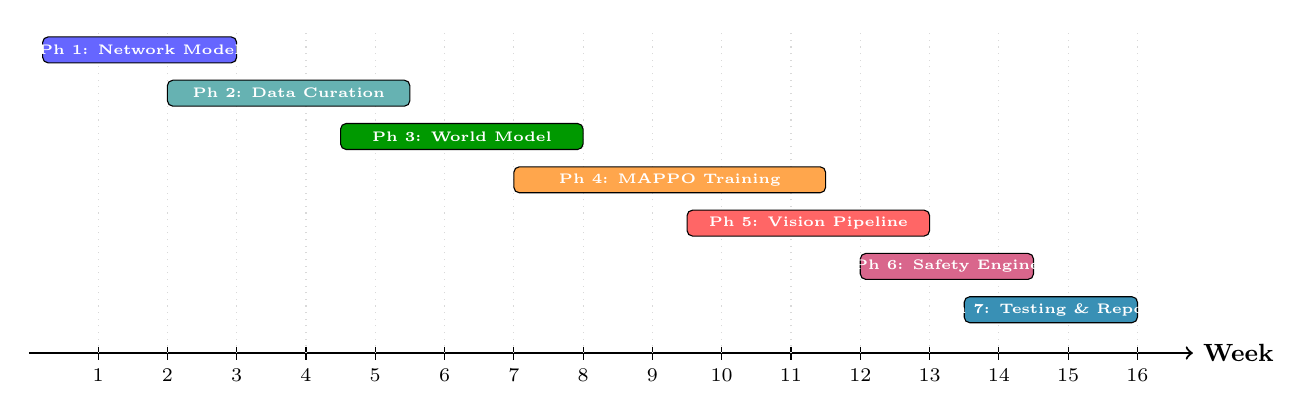
\begin{tikzpicture}[x=0.88cm, y=0.55cm]
    % Timeline grid
    \draw[->, thick] (0,0) -- (16.8,0) node[right, font=\small\bfseries] {Week};
    \foreach \w in {1, 2, ..., 16} {
        \draw (\w, 0.15) -- (\w, -0.15) node[below, font=\scriptsize] {\w};
        \draw[dotted, gray!30] (\w, 0) -- (\w, 7.5);
    }
    
    % Tasks
    \draw[fill=blue!60, rounded corners=2pt] (0.2, 6.7) rectangle (3.0, 7.3) node[midway, white, font=\tiny\bfseries] {Ph 1: Network Model};
    \draw[fill=teal!60, rounded corners=2pt] (2.0, 5.7) rectangle (5.5, 6.3) node[midway, white, font=\tiny\bfseries] {Ph 2: Data Curation};
    \draw[fill=green!60!black, rounded corners=2pt] (4.5, 4.7) rectangle (8.0, 5.3) node[midway, white, font=\tiny\bfseries] {Ph 3: World Model};
    \draw[fill=orange!70, rounded corners=2pt] (7.0, 3.7) rectangle (11.5, 4.3) node[midway, white, font=\tiny\bfseries] {Ph 4: MAPPO Training};
    \draw[fill=red!60, rounded corners=2pt] (9.5, 2.7) rectangle (13.0, 3.3) node[midway, white, font=\tiny\bfseries] {Ph 5: Vision Pipeline};
    \draw[fill=purple!60, rounded corners=2pt] (12.0, 1.7) rectangle (14.5, 2.3) node[midway, white, font=\tiny\bfseries] {Ph 6: Safety Engine};
    \draw[fill=cyan!70!black, rounded corners=2pt] (13.5, 0.7) rectangle (16.0, 1.3) node[midway, white, font=\tiny\bfseries] {Ph 7: Testing \& Report};
\end{tikzpicture}
\caption{Gantt chart of the 16-week project execution timeline}
\label{fig:ch1_gantt}
\end{figure}

\subsection{Roles and Responsibilities}
Table \ref{tab:roles_responsibilities} outlines the assignment of engineering responsibilities across the modular project architecture.

\begin{table}[htbp]
\centering
\small
\caption{Roles and responsibilities for system design and execution}
\label{tab:roles_responsibilities}
\begin{tabularx}{\textwidth}{|p{3.5cm}|X|p{4.2cm}|}
\hline
\textbf{Role / Module} & \textbf{Core Technical Responsibilities} & \textbf{Deliverables} \\ \hline
Perception \& Vision & YOLOv8 integration, BMD-45 taxonomy mapping, LAP tracking, stationary queue filters & \texttt{live\_vision\_pipeline.py}, video processing engine \\ \hline
Dynamics \& World Model & Dataset ingestion, transition synthesis, residual multi-task network design & \texttt{neural\_world\_model.py}, \texttt{train\_world\_model.py} \\ \hline
Multi-Agent RL Control & MAPPO algorithm, Actor-Critic networks, CTDE logic, GAE advantage calculation & \texttt{mappo\_networks.py}, \texttt{train\_mappo\_data\_driven.py} \\ \hline
Environment \& Safety & Gymnasium environment, dual-ring signal state machine, min-green \& yellow locks & \texttt{data\_driven\_env.py}, signal safety constraints \\ \hline
User Interface \& Testing & Streamlit interactive dashboard, OpenCV HUD actuator, 6-scenario benchmarking & \texttt{dashboard\_live\_vision.py}, \texttt{live\_traffic\_controller.py} \\ \hline
Project Supervision & Architecture evaluation, milestone review, technical verification & Review feedback, validation sign-off \\ \hline
\end{tabularx}
\end{table}

\subsection{Challenges and Risk Management}
Deploying deep reinforcement learning and computer vision to safety-critical municipal infrastructure involves substantial operational and theoretical risks. Table \ref{tab:risk_register} enumerates the primary identified risks and the structural engineering mitigations incorporated into the system design.

\begin{table}[htbp]
\centering
\small
\caption{Project risk register and mitigation strategies}
\label{tab:risk_register}
\begin{tabularx}{\textwidth}{|p{3.2cm}|c|c|X|}
\hline
\textbf{Identified Risk} & \textbf{Impact} & \textbf{Likelihood} & \textbf{Mitigation Strategy} \\ \hline
Sim-to-Real Discrepancy & High & High & Calibrated dynamics using 40 days of empirical 1-second interval IIT Delhi queue measurements and Pune vehicle splits. \\ \hline
Sim Rapid Phase Flutter & Critical & Medium & Hardcoded minimum green interval ($12\text{ s}$) in state machine preventing RL policy from erratic switching. \\ \hline
TraCI Socket Crashes & High & High & Developed standalone PyTorch Neural World Model (\texttt{data\_driven\_env.py}), achieving 100\% simulator independence. \\ \hline
Downstream Gridlock & High & Medium & Centralized Critic observes global 66-dim corridor state, penalizing upstream agents for dumping traffic into choked links. \\ \hline
Edge Vision Latency & Medium & Medium & Selected lightweight YOLOv8 Nano (\texttt{yolov8n.pt}, 6.2 MB) running in quantized CPU mode, sustaining $\ge 30$ FPS. \\ \hline
\end{tabularx}
\end{table}

\section{Scope and Limitations}
\label{sec:scope_limitations}

\subsection{In Scope}
The boundaries of this project encompass:
\begin{enumerate}
    \item Modeling and simulating a 3-intersection coordinated arterial corridor based on the geometry of the NH-48 Delhi--Gurgaon Expressway.
    \item Multi-Agent Proximal Policy Optimization with decentralized Actor policies and a centralized corridor Critic.
    \item Edge computer vision inference on video and camera feeds classifying Two-Wheelers, Auto-Rickshaws, Passenger Cars, Buses, and Commercial Trucks.
    \item Empirical Passenger Car Unit (IRC:106) cost formulations integrated into the reinforcement learning reward function.
    \item Standalone, simulator-free Neural Traffic World Model operating as an execution and evaluation digital twin.
    \item Live OpenCV video HUD actuator and interactive Streamlit web telemetry dashboard.
\end{enumerate}

\subsection{Out of Scope}
The following aspects are deliberately excluded and reserved for future research:
\begin{enumerate}
    \item Direct physical wiring and relays into roadside municipal electromechanical traffic control cabinets (the prototype interfaces via software telemetry and visual HUD actuators).
    \item City-wide macroscopic grid networks beyond linear arterial corridors.
    \item V2X (Vehicle-to-Everything) dedicated short-range wireless communications directly into onboard connected vehicle units.
\end{enumerate}

\subsection{System Limitations}
\begin{itemize}
    \item \textbf{CCTV Occlusion in Dense Crowds}: Extreme congestion can cause visual occlusion where larger commercial trucks partially obscure trailing two-wheelers.
    \item \textbf{Lighting Extremes}: Optical detection accuracy under dense nocturnal fog or heavy torrential monsoon rain is subject to camera sensor limitations.
    \item \textbf{Fixed Model Topologies}: The neural world model is currently calibrated to 8 incoming and 4 outgoing lanes per junction.
\end{itemize}
